\documentclass[tikz]{standalone}

\usetikzlibrary{arrows, automata, positioning}

\begin{document}

        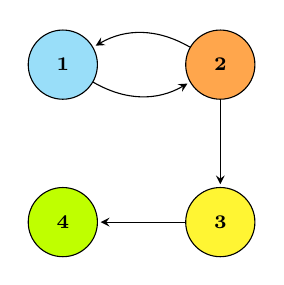
\begin{tikzpicture}[>=stealth, shorten >=1pt,node distance=2cm,on grid,auto, initial text = {}]

        \tikzstyle{every state}=[fill={rgb:black,1;white,10}]

        \node[state, fill=cyan!40]   (q_1) {\scriptsize $\textbf{1}$};
        \node[state, fill=orange!70]   (q_2) [right of =q_1] {\scriptsize $\textbf{2}$};
        \node[state, fill=yellow!80]   (q_3) [below of =q_2] {\scriptsize $\textbf{3}$};
        \node[state, fill=lime]   (q_4) [left of =q_3] {\scriptsize $\textbf{4}$};


        \path[->]
        (q_1) edge  [bend right, above] (q_2)
        (q_2) edge  [bend right, above] (q_1)
        (q_2) edge   (q_3)
        (q_3) edge   (q_4);

        \end{tikzpicture}

\end{document}